\subsection{Modelo de compactación y acoplamiento}
\label{app:prototipo_A3}
Se emplea exclusivamente el prototipo definitivo y biomasa de 4\,mm.
La identidad geométrica de la matriz se contrastó por volumen, 102 centros
y muestreo bidireccional de frontera, con tolerancia $10^{-5}$ mm.
El radio de cada rodillo es 26\,mm, su ancho radial 30\,mm, sus centros están
a 27,75\,mm del eje principal y la separación inicial es 0,5\,mm.
El marco de cálculo se alinea con el eje transversal real, girado 30grados
respecto del eje globalX; no se usan sus cajas envolventes como longitudes.
\begin{align}
 P&=\frac{P_{N0}}{\nu_{LR}}\left[\exp\left(4\mu_p\nu_{LR}L/D\right)-1\right],\\
 P_{N0}&=0,281\ {\rm MPa},\quad\nu_{LR}=0,203,\quad\mu_p=0,715,
 \quad L/D=10/6,\quad P=2,25867\ {\rm MPa}.
\end{align}
Los coeficientes y el procedimiento se conservan de EP2
\cite{equipo_entrega2_2026}; esta presión es una estimación de diseño,
no una calibración experimental de aserrín.

\subsubsection*{Áreas y centroides corregidos}
Para cada abscisa radial $r$, se recorta el segmento circular mediante
$t_-=\max(t_c-\sqrt{a^2-(r-r_c)^2},-L_c/2)$ y
$t_+=\min(t_c+\sqrt{a^2-(r-r_c)^2},L_c/2)$, donde $a=3$ mm.
El ancho de huella conserva la ley empleada en el modelo previo:
\begin{equation}
 L_c(g)=\sqrt{D_R(h-g)-(h-g)^2},\qquad h=4\ {\rm mm}.
\end{equation}
Con $\ell=\max(t_+-t_-,0)$ y pesos de Gauss $w_k$:
\begin{align}
 \widetilde A&=\sum_k w_k\ell_k,\qquad A=\min(\widetilde A,\pi a^2),\\
 \bar r&=\frac{\sum_k w_k r_k\ell_k}{\widetilde A},\qquad
 \bar t=\frac{\tfrac 12\sum_k w_k(t_{+,k}^2-t_{-,k}^2)
 \mathbf 1_{\ell_k>0}}{\widetilde A}.
\end{align}
La corrección anula el primer momento de intervalos vacíos. La
normalización del centroide usa el área integrada antes de su recorte
numérico al área circular; el área de fuerza continúa limitada por
$\pi a^2$. Para $A=0$ el centroide no se usa. La implementación corregida
es una versión separada; el código histórico permanece intacto.
Se verificó en los 1440 estados que todo centroide positivo pertenece
al disco y a la huella recortada. Se contrastaron simetría, contacto nulo
y el centroide analítico de un semidisco.

\subsubsection*{Iteración geométrica--estructural}
Para cada ángulo se recalculan $F_{ij}=PA_{ij}$ y
$T=0,1\sum_{ij}r_iF_{ij}$, manteniendo el radio de perforación empleado
por EP2. El reparto entre 608 conserva fuerzas y primeros momentos.
La viga de Euler--Bernoulli devuelve desplazamientos y pendientes, y
$g_j(r)=g_0+u_j+\alpha_j(r-r_j)$ actualiza la huella.
Se mantiene relajación 0,5, tolerancia de holgura $10^{-9}$ m, cambio relativo
de fuerza $10^{-5}$ y máximo 100 iteraciones. La solución se reevalúa antes
de aceptar convergencia. No se fuerza coincidencia con resultados previos.
\begin{center}\begin{tabular}{ll}\toprule
Resultado & Valor\\\midrule
Estados convergidos & 1440/1440\\
Iteraciones máximas & 18\\
Fuerza máxima & 918,062 N\\
Fuerza media & 900,640 N\\
Torque máximo & 2,779984 N\,m\\
Torque medio & 2,666731 N\,m\\
\bottomrule\end{tabular}\end{center}

Los máximos de fuerza y torque corresponden a estados distintos;
se conservan las series completas y se evita mezclarlos al verificar.
Los contrastes de cuadratura 128 y malla de viga 160 divisiones se ejecutan
en 32 estados con inicio independiente. Sus errores se documentan en
\texttt{validacion\_numerica\_3C.csv}; el error de discretización no debe
confundirse con el residuo de convergencia de una iteración.
\begin{center}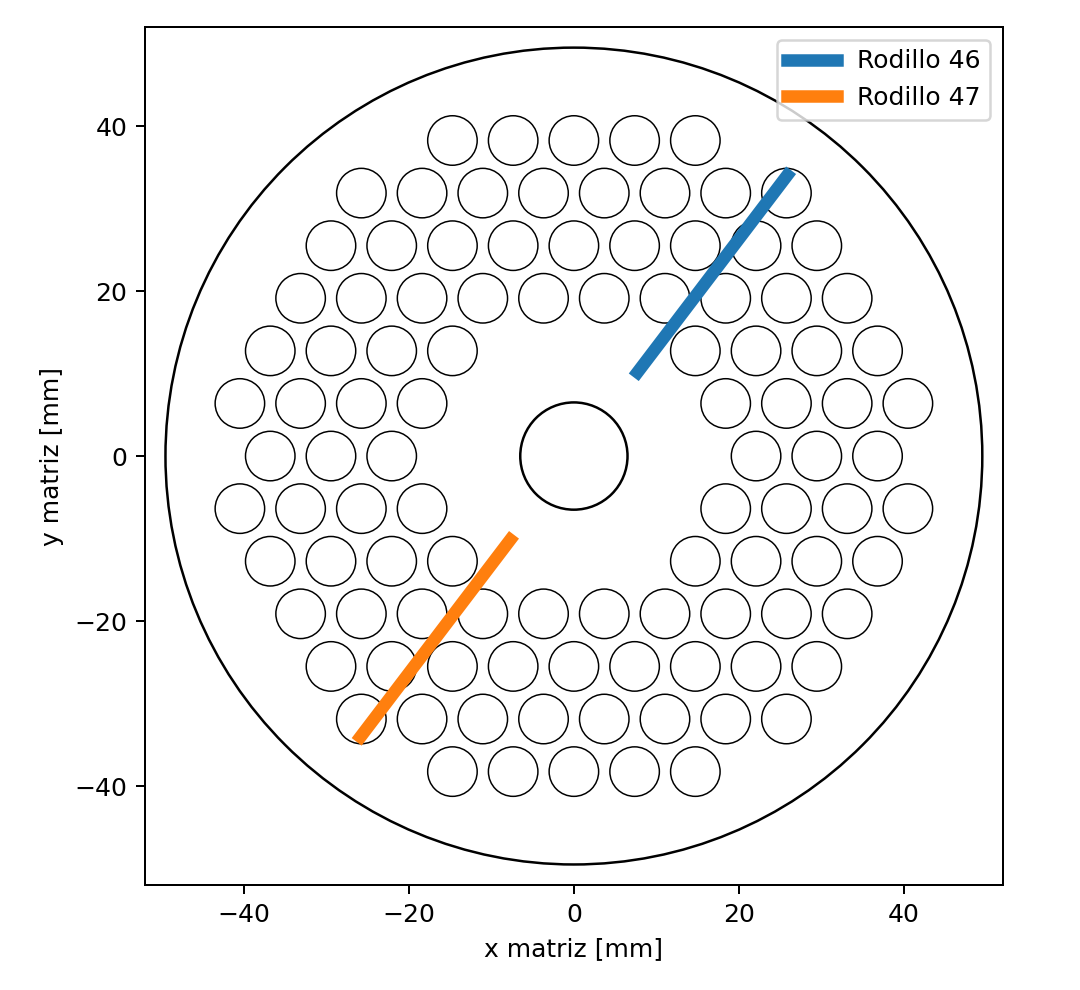
\includegraphics[width=.65\linewidth]{geometria_contacto.png}\end{center}
\begin{center}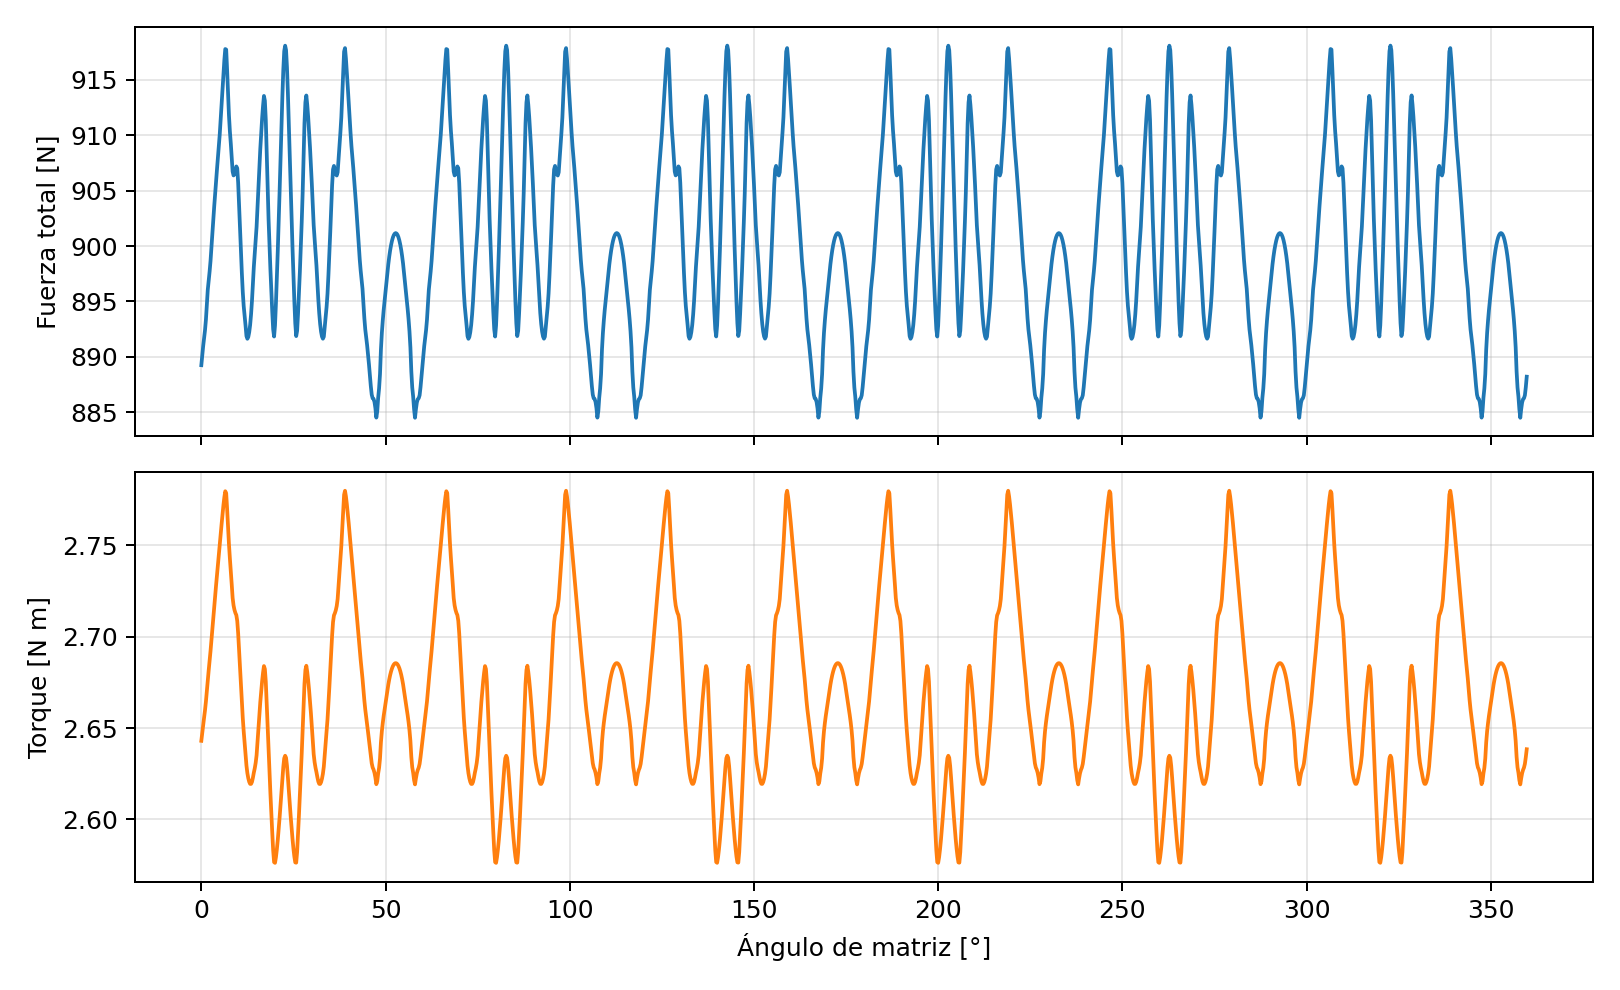
\includegraphics[width=.85\linewidth]{fuerzas_torque.png}\end{center}
